\documentclass[a4paper, 12pt]{article}
\usepackage[utf8]{inputenc}
\renewcommand\familydefault{\sfdefault}
\usepackage[T1]{fontenc}
\usepackage[francais]{babel}
\usepackage[left=2cm,top=2cm,right=2cm,bottom=2cm]{geometry}
\usepackage{graphicx}
\usepackage{minted}
\usemintedstyle{colorful}
\usepackage{float}
\floatplacement{figure}{H}
\usepackage{authblk}
\usepackage{enumitem}
\usepackage{hyperref}
\hypersetup{
	colorlinks,
	citecolor=black,
	filecolor=black,
	linkcolor=black,
	urlcolor=blue
}

\usepackage{caption}
\newenvironment{code}{\captionsetup{type=listing}}{}

\begin{document}

\title{Doge FS}
\author{Raed Abdennadher et Steven Liatti}
\affil{\small Programmation avancée des systèmes - Prof. Florent Glück}
\affil{\small Hepia ITI 3\up{ème} année}
\maketitle

% \tableofcontents
% \listoffigures
% \renewcommand\listoflistingscaption{Table des listings de code source}
% \listoflistings

\section{Description}
Ce rapport décrit le système de fichiers "Doge FS" utilisé dans notre kernel. Doge FS est basé sur
\href{https://en.wikipedia.org/wiki/File_Allocation_Table}{File Allocation Table (FAT)}, un système
de fichier très répandu. Une image formatée en Doge FS contient des blocs de bytes (multiple de 512).
Les tous premiers bytes d'une image (situés dans le premier bloc) contiennent les informations de base
du système, nous l'appelons le "super bloc". Le(s) bloc(s) suivant(s) contien(nen)t la FAT, un tableau de
listes chainées d'indices de blocs. Finalement, après la FAT, les blocs suivants contiennent soit des
méta-données (des "entrées") des fichiers, soit les données proprement dites des fichiers. Ce système
est non hiérarchique (pas de gestion des dossiers), tous les fichiers sont à la "racine".
Voici le détail des 3 structures de données mentionnées ci-dessus :
\begin{itemize}
	\item \mintinline{c}{super_block_t} : contient les informations de base du système :
	\begin{itemize}
		\item \mintinline{c}{magic} : (\mintinline{c}{char}) la signature, à 0x42, ou 66 en base 10
		\item \mintinline{c}{version} : (\mintinline{c}{char}) la version du système
		\item \mintinline{c}{label} : tableau de \mintinline{c}{char} contenant le nom du système (ici "doge\_os")
		\item \mintinline{c}{block_size} : (\mintinline{c}{int}) la taille d'un bloc (multiple de 512, jusqu'à 4096)
		\item \mintinline{c}{fat_len} : (\mintinline{c}{int}) le nombre total de blocs indexés par la FAT (= nombre de blocs total)
		\item \mintinline{c}{fat_block_nb} : (\mintinline{c}{int}) le nombre de blocs occupés par la FAT elle-même
		\item \mintinline{c}{first_entry} : (\mintinline{c}{int}) l'indice du premier bloc de méta-données
	\end{itemize}
	\item \mintinline{c}{entry_t} : représente les méta-données, c'est une liste d'entrées de fichiers :
	\begin{itemize}
		\item \mintinline{c}{name} : tableau de \mintinline{c}{char} contenant le nom du fichier
		\item \mintinline{c}{size} : la taille en bytes du fichier
		\item \mintinline{c}{start} : l'indice du premier bloc de données du fichier
	\end{itemize}
	\item FAT : tableau de \mintinline{c}{int}. Chaque case représente un bloc du système de fichier et contient :
	\begin{itemize}
		\item -1 : indique que le bloc est libre et n'a pas de suivant
		\item 0 : indique que ce bloc est le dernier d'une liste chainée de données ou de méta-données
		\item entier compris entre 2 et $fs_{size} / block_{size}$ : indique l'indice du bloc suivant de données ou de méta-données
	\end{itemize}
\end{itemize}
Le schéma suivant représente un exemple de disposition des structures et données sur une image Doge FS :
\begin{figure}
	\begin{center}
		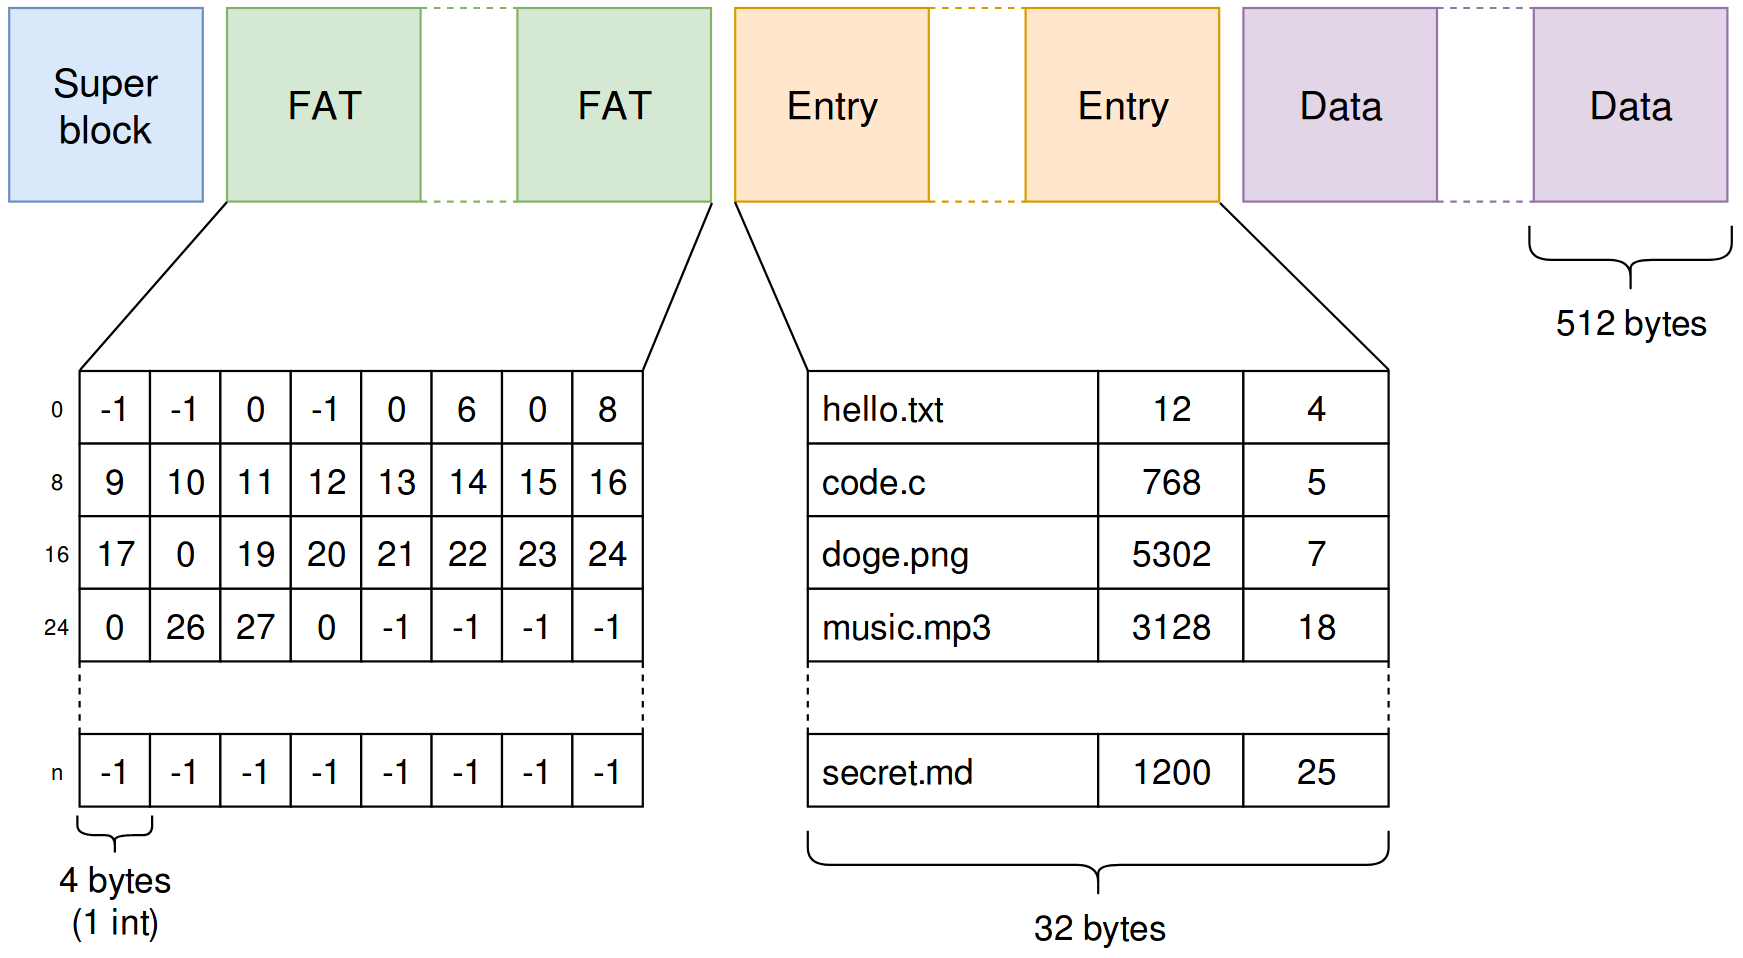
\includegraphics[width=1.0\textwidth]{schema.png}
		\caption{Format du système de fichiers}
	\end{center}
\end{figure}
Sur ce schéma, les blocs ont une taille de 512 bytes. Avec une taille maximale de label fixée à 20 caractères,
le super bloc a une taille constante de 38 bytes, quelle que soit la taille de bloc choisie. Le sous-tableau de
gauche représente la FAT. Elle occupe au minimum un bloc et commence au bloc 1 (ici à un offset de 512 bytes).
La FAT peut contenir $block_{size} / 4$ cases par bloc, ici 128. Sur le schéma, les numéros positionés à gauche de la
FAT représentent les indices des cases. Les deux premières cases sont à -1, elles représentent respectivement
le super bloc et la première case de la FAT elle-même.
Le sous-tableau de droite représente la liste des entry (les méta-données). Avec une longueur maximale de 24
caractères pour un nom de fichier, une entrée a une taille de 32 bytes (24 bytes de nom, 4 bytes de taille et
4 bytes d'indice de premier bloc de données), par conséquent un bloc de 512 bytes peut en contenir 16 
($block_{size} / 32$).
\\
Dans cet exemple, 2 blocs sont alloués pour les méta-données, les blocs 2 et 3. 
Le premier fichier, "hello.txt" occupe un bloc et se trouve à l'indice 4, qui contient un zéro, indiquant 
qu'il s'agit de la fin de la chaine. Le deuxième fichier, "code.c" occupe 2 blocs, aux indices 5 et 6 dans la FAT.
Les autres fichiers remplissent la FAT en séquence selon la même analogie.
À noter qu'une fois passés les blocs de FAT, le prochain bloc sera un bloc d'entry, mais les suivants pourront
contenir soit des entry, soit des données de fichiers. Cette alternance est possible grâce à la structure 
de liste chainée qui est en place dans la FAT. Cela apporte plus de souplesse lorsque de nombreux fichiers 
sont ajoutés.
\\
Lorsque le kernel est exécuté avec une image Doge FS montée comme système de fichiers, nous chargeons en 
mémoire vive toute la FAT, pour obtenir directement les indices des blocs à lire/écrire sur le disque. Étant 
donné que l'écriture de fichiers côté kernel n'est pas requise dans ce TP, la FAT en RAM sera la seule à être 
consultée. Si nous devions gérer les cas d'écriture, nous pourrions imaginer un mécanisme d'écriture intermittente
qui mettrait à jour la FAT sur le disque lorsque nécessaire.

% TODO: enlever numéros du tab entry et changer un peu ordre dans la FAT

\newpage
\section{Avantages et inconvénients}
\subsection{Avantages}
\begin{itemize}
	\item Implémentation aisée
	\item Les fichiers peuvent facilement grandir
	\item Pas de fragmentation externe
	\item Accès aléatoire rapide, grâce à la FAT chargée en RAM
\end{itemize}
\subsection{Inconvénients}
\begin{itemize}
	\item Overhead important pour le stockage de la FAT (disque et RAM)
	\item Accès séquentiel potentiellement lent, bien que limité dans notre cas
\end{itemize}

\end{document}
